\chapter{Network Flow Monitoring}\label{chap:network-flow-monitoring}

\begin{chapintro}

Flow monitoring is an important part of network accounting and security nowadays. It facilitates large scale intrusion detection and prevention systems, data analysis, capacity planning, data retention, and other operations important for network management. The aim of this chapter is to provide a comprehensive introduction to network flow monitoring. Firstly, the history of flow monitoring is outlined and related technologies are described and compared to flow monitoring. Secondly, the applicability of currently used flow definitions is discussed and an improved definition is proposed, together with a formal notation. The formal notation allows clear description of flow related algorithms and avoids misunderstandings caused by ambiguities of a natural language. To the best of our knowledge, this is the first attempt to formalise the flow creation process that takes into account all input data used in practice. The rest of the chapter presents the flow monitoring process in detail. Issues encountered while deploying and operating flow monitoring infrastructure of CESNET National Research and Education Network are discussed at the end of this chapter. 

With an exception of the novel flow definition, this chapter covers similar topic as the article of \citeauthor{Hofstede-2014-Flow}~\cite{Hofstede-2014-Flow}. The article served as one of the sources of information about history of flow monitoring and as an inspiration for the structure of this chapter. The reader is encouraged to study the article as an additional source of information. It focuses more on the IPFIX protocol and contains extensive information about the capabilities of existing enterprise and open-source software for flow creation and processing. 

%The main contribution of this chapter is the improved flow definition together with its formal notation and formal description of the flow creation process.

The organisation of this chapter is as follows:
\begin{itemize}
  \item Section~\ref{sec:flow-monitoring-basics} introduces flow monitoring and provides overview of its history and related technologies.
  \item Section~\ref{sec:flow-definition} provides an improved flow definition and based on this definition provides formal description of flow creation process.
  \item Section~\ref{sec:flow-monitoring-architecture} explains flow monitoring architecture.
  \item Section~\ref{sec:flow-monitoring-process} describes the flow monitoring process from packet capture to flow record export.
  \item Section~\ref{sec:flow-data-processing} describes flow data treatment from flow record reception to storage and further processing.
  \item Section~\ref{sec:common-issues} discusses common issues encountered in flow monitoring operation.
  \item Section~\ref{sec:nfm-conclusions} concludes the chapter.
\end{itemize}

\end{chapintro}

% \todo{Do not start with the reference. Rewrite first paragraph, there is much added value here}
% The article of \citeauthor{Hofstede-2014-Flow}~\cite{Hofstede-2014-Flow} extensively covers the topic of flow monitoring process and much information provided in this chapter is influenced by it. The reader is encouraged to study the article, the relevant sections are II to VIII with the exception of section VII. However, this chapter explains the flow monitoring process in the context of this thesis, therefore some aspects of the flow monitoring, such as flow export processes, are described in more detail.

\newpage

\section{Flow Monitoring Basics}\label{sec:flow-monitoring-basics}

This section describes history and current state of network flow monitoring. We discuss related standards, introduce terminology used throughout this thesis and provide formal definition of a flow. 

\subsection{History of Flow Monitoring}\label{subsec:history-of-flow-monitoring}

The first mention of a flow export can be found in RFC 1272~\cite{rfc1272} published in 1991 by IETF Internet Accounting (IA) Working Group (WG). The goal of the document was to provide background information on Internet accounting. The authors describe methods of metering and reporting network utilization. The RFC defines a metering process as follows:

\begin{displaycquote}{rfc1272}[Internet accounting: Background]
A METER is a process which examines a stream of packets on a communications medium or between a pair of media. The meter records  aggregate counts of packets belonging to FLOWs between communicating entities (hosts/processes or aggregations of communicating hosts (domains)).
\end{displaycquote}

The goal at the time was to provide a framework for traffic accounting, however, the common believe at the time was that internet should be free and any form of traffic capture, even for the accounting purposes, is undesirable. This, together with the lack of vendor interest, resulted in the conclusion of the working group in 1993. Note that the negative attitude towards the monitoring returns more than 20 years later~\cite{rfc7258}.

In 1995, \citeauthor{Claffy-1995-Parameterizable} showed a methodology for internet traffic flow profiling based on packet aggregation~\cite{Claffy-1995-Parameterizable}, which started a revival of flow monitoring efforts. The Realtime Traffic Flow  Measurement (RTFM) Working Group was created in 1996 and it had three main objectives. First was to consider current issues relating to traffic measurement, such as security, privacy, policies and requirements on new network protocols. Second was to produce an improved Traffic Flow Model that should provide a wider range of measurable quantities (e.g. IPv6), simpler way to specify flows of interest, better access control  to measured flow data, strong focus on data reduction capabilities and efficient hardware implementation. The third objective was to develop RTFM Architecture and Meter Management Information Base (MIB) as a standards track IETF documents. The effort resulted in 1999 by publishing several RFCs describing new traffic flow measurement framework with an increased flexibility and even a bi-directional flow support~\cite{rfc2722}. Since these documents fulfilled the objectives of the RTFM WG, the group was concluded in 2000. However, no flow export standard was developed as the vendors showed no interest in this area.

Meanwhile, Cisco realized that similar kind of flow information is already stored in a flow cache of their packet switching devices. The purpose of this cache is to speed up packet switching by making a forwarding decision only for the first packet of each flow. Unlike the RTFM flow measurement framework, the primary purpose of flow cache is not accounting nor monitoring, therefore the configuration of measurement process using a flow cache in a switch is severely limited. Despite the limitations, once Cisco introduced its own flow export technology called \Index{NetFlow}, it achieved widespread adoption. The main reason for the extensive adoption was the fact that it was readily available in most Cisco devices with little effort. The NetFlow was patented in 1996 and the first version that became available to general public around 2002 was NetFlow v5~\cite{CiscoSystems-2007-NetFlow}, albeit Cisco newer released any official specification. The NetFlow v5 format simply specified a single set of fields that should be exported from each flow record. Figure~\ref{fig:nf5-fields} shows all fields that were supported by NetFlow v5. Note the lack of support for IPv6 protocol.

\begin{figure}[t!]
  \begin{center}
    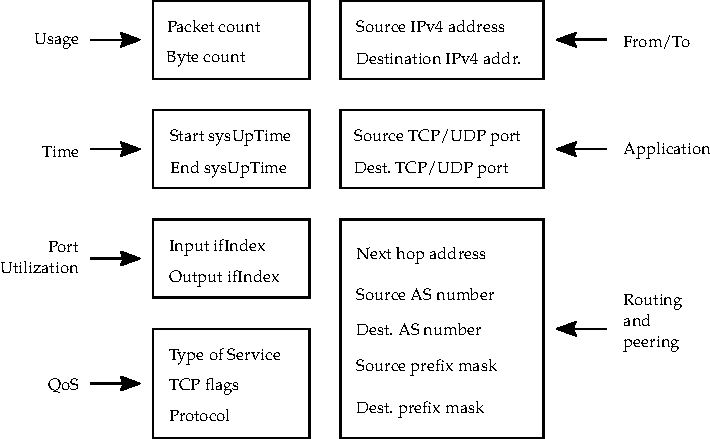
\includegraphics{figures/nf5-fields}
  \end{center}
  \caption{Fields exported by NetFlow v5~\cite{CiscoSystems-2007-NetFlow}.}
  \label{fig:nf5-fields}
% http://www.cisco.com/c/dam/en/us/td/i/000001-100000/60001-65000/60001-61000/60682.ps/_jcr_content/renditions/60682.jpg
\end{figure}

The NetFlow version 5 was soon obsoleted by NetFlow version 9 which remedied some of the deficiencies of the previous version. The state of NetFlow v9 is described in~\cite{rfc3954}. It allowed to define arbitrary set of fields for export using templates as shown in Figure~\ref{fig:nf9-protocol}. It also introduced support for new protocols, such as IPv6, Virtual Local Area Networks (VLAN), Multiprotocol Label Switching (MPLS), Border Gateway Protocol (BGP) or Multicast. 

\begin{figure}[t!]
  \begin{center}
    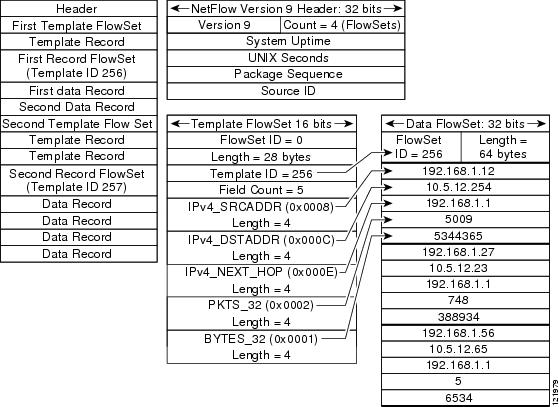
\includegraphics[width=\textwidth]{figures/nf9-protocol}
  \end{center}
  \caption{NetFlow~v9 protocol structure example~\cite{CiscoSystems-2007-NetFlow}.}
  \label{fig:nf9-protocol}
% http://www.cisco.com/c/dam/en/us/td/i/100001-200000/120001-130000/121001-122000/121979.ps/_jcr_content/renditions/121979.jpg
\end{figure}

Other vendors created their own versions of flow exporting protocols, although they retained some level of compatibility with NetFlow. There are JFlow by Juniper, CFlow by Alcatel-Lucent, RFlow by Ericsson, and other protocols. When the potential of flow monitoring for security purposes became realized in 2005~\cite{CiscoSystems-2005-Cisco}, more effort was devoted to extend flow records with information not directly associated with switching. Cisco presented Flexible NetFlow technology~\cite{CiscoSystems-2008-Cisco} in 2006 which allows to dynamically define and export new types of information, such as parts of payloads or traffic identification.

In 2001, it was clear that exporting flow information from switching devices is going to be supported by vendors. However, no standard flow export protocol existed at the time and NetFlow v5 was not yet released to general public. For that reason the IETF started \Index{IP Flow Information Export} (\Index{IPFIX}) WG~\cite{IETF--IP}. The original charter~\cite{IESG-2001-IP} defined six specific goals for the WG: 

\begin{itemize}
	\item Define \emph{``standard IP flow''}.
	\item Devise flow data encoding that support multiple levels of aggregation.
	\item Allow packet sampling in IP flow.
	\item Identify and address security and privacy concerns affecting flow data.
	\item Specify the transport mapping for IP flow information.
	\item Ensure that the flow export system is reliable.
\end{itemize}

The charter was updated over the years to match current requirements. Several vendors were engaged in the IPFIX WG’s activities, most notably Cisco, which significantly contributed from the start. The WG defined set of requirements for the IPFIX protocol~\cite{rfc3917} and evaluated existing candidate protocols~\cite{rfc3955} to decide the most suitable approach in defining the new protocol. The NetFlow v9 specification (RFC 3954) was designed with IPFIX requirements in mind~\cite{Trammell-2011-Introduction} and was released in order to compete in this evaluation (RFC 3955). After the evaluation the NetFlow v9 was chosen as a basis of the new IPFIX protocol. For this reason, the IPFIX is sometimes called NetFlow v10 and even starts with protocol version 10 in its header. However, the IPFIX protocol supports many new features and is not completely backwards compatible with NetFlow.

The IPFIX WG did more than just design the IPFIX protocol. In the 29 RFCs submitted before its conclusion, the WG paid attention to e.g.:
\begin{itemize}
	\item Bidirectional flow export~\cite{rfc5103}
	\item Architecture for IP flow information export~\cite{rfc5470}
	\item Reducing redundancy in flow~\cite{rfc5473}
	\item Definitions of Managed Objects (MIB) for IPFIX~\cite{rfc5815, rfc6615, rfc8038}
	\item IP flow mediation framework~\cite{rfc5982, rfc6183}
	\item IP flow anonymization~\cite{rfc6235}
	\item IPFIX configuration data model~\cite{rfc6728}
\end{itemize}
The IPFIX protocol specification is described by \emph{``Specification of the IP Flow Information Export (IPFIX) Protocol for the Exchange of Flow Information''}~\cite{rfc7011} which became an Internet Standard. The working group was concluded in 2014, however, IPFIX related Internet-Drafts are still being created by involved parties. Further information about IPFIX development is provided by \citeauthor{Brownlee-2011-Flow} in \cite{Brownlee-2011-Flow}.

\subsection{Related Technologies}

Flow monitoring is not the only network monitoring system used to gain information about network behavior. There are other technologies that can be used to monitor network traffic and that can be sometimes confused with flow monitoring. We describe \Index{sFlow}~\cite{Phaal-2004-sFlow}, \Index{IETF Packet Sampling}, \Index{OpenFlow} and Deep Packet Inspection\index{deep packet inspection} in the following text.

sFlow is an industry standard that is supported by number of vendors in their packet switching devices. Its initial specification was published as an Informational RFC~\cite{rfc3176} in 2001, which was the time when packet switching/routing devices with sFlow support became available. The most crucial difference from flow monitoring is that the sFlow does not actually aggregate a stream of packet into a flow record. Instead, it uses sampling to select individual packets and then exports information available about and from these packets. sFlow allows to export data from packet headers, chunks of data from packets and even parse application payloads. It also maintains interface counters and allows their regular export, which is a feature completely unrelated to flow monitoring. sFlow version 5 is the latest version and was published in~\citeyear{Phaal-2004-sFlow}~\cite{Phaal-2004-sFlow}.

In 2002 the IETF started Packet Sampling (PSAMP) Working Group~\cite{IETF--Packet} which was chartered to define a standard set of capabilities for network elements to sample subsets of packets by statistical and other methods~\cite{IESG--Packet}. The result is similar to sFlow, however, the PSAMP uses IPFIX protocol for data export~\cite{rfc5477}. The WG was concluded in 2009 after publishing four RFCs. The proposed standards include sampling and filtering techniques for IP packet selection~\cite{rfc5475}, packet sampling protocol specifications~\cite{rfc5476} and information model for packet sampling export~\cite{rfc5477}.

OpenFlow~\cite{ONF-2012-OpenFlow} is an open-source implementation of the Software Defined Networking (SDN) concept~\cite{Singh-2017-Survey, Hu-2014-Survey}. The idea of SDN is to separate control plane and data plane of networking devices. This means that the packet forwarding rules are known only to SDN controllers. The other networking devices that process the traffic ask the controllers what to do with individual flows. After the decision is made for the first packet of the flow, a flow record is kept in the cache so that subsequent lookups do not require the controller interaction. The OpenFlow is a protocol of communication between the networking devices and the controllers. It has been shown by \citeauthor{Yu-2013-FlowSense}~\cite{Yu-2013-FlowSense} that the information stored in the flow caches can be exported using the OpenFlow protocol to the controller and used for network monitoring. Although the approach to network monitoring is somewhat similar to flow monitoring on non-SDM networking devices, there are significant differences. The control traffic itself is utilized to transfer data about new and expired flow records. Therefore, configuration of flow monitoring is directly affected by configuration of SDN network and vice versa. This imposes undesirable restrictions on the flow monitoring process. Moreover, the distributed architecture of the monitoring is tightly coupled with the deployment of the network controllers. For these reasons, this thesis does not consider SDN specific flow monitoring. It should be noted, that the SDN enabled networking devices can still export valid flow data as defined by the IPFIX standard. In such a case, the SDN capabilities are irrelevant for flow monitoring purposes.

% TODO Add paper ``Towards a NetFlow implementation for OpenFlow Software-Defined Networks'' (https://itc29.org/en/program/conference-program.html)

Deep Packet Inspection (DPI) is an approach to network data analysis where each packet is dissected up to and including application layer protocol (i.e. packet payload). Although this requires much greater resources than standard flow monitoring, it provides maximum information about network traffic. DPI is an approach, rather than a specific technology, therefore the means of packet capture and information export depend on the particular deployment. For example, sFlow uses DPI to gain information about application layer from packet payloads and exports this information as part of the sFlow protocol. Despite the DPI being diametrically different to flow monitoring, it is being integrated to flow monitoring process to provide the application visibility. This merge balances the detailed view of DPI with the fast and scalable architecture of the flow monitoring. This thesis describes how the DPI is integrated to flow monitoring to create Application Flow Monitoring. Neither sFlow nor OpenFlow are not discussed any further in this work and PSAMP is only mentioned as a packet sampling protocol that can be optionally applied to flow monitoring.


\section{Flow Definition}\label{sec:flow-definition}

To be able to accurately describe the flow monitoring process, we need to have a precise definition of what a flow is. The NetFlow v9 description in~\cite{rfc3954} uses the following definition:

\begin{displaycquote}{rfc3954}[Cisco Systems NetFlow Services Export Version 9]

    An IP Flow, also called a Flow, is defined as a set of IP packets
    passing an Observation Point in the network during a certain time
    interval. All packets that belong to a particular Flow have a set of
    common properties derived from the data contained in the packet and
    from the packet treatment at the Observation Point.

\end{displaycquote}

The Observation Point is defined as a location where IP packets can be observed. The definition says that a flow is a set of packets within certain time span. Furthermore, the packets in a flow have a set of common properties and these properties are either derived from data contained in the packet data or from packet treatment (e.g. next hop IP address or input interface). Although this definition is quite generic, it covers most of the common IP flow creation techniques.

The IPFIX Protocol is an internet standard~\cite{rfc7011} with its own definition of a flow that builds upon the NetFlow v9 definition. It tries to specify what “properties derived from data contained in packet data” means and differentiates two types of data. The first are the values contained in packet headers, the second type covers the characteristics of the packet itself (e.g. packet length). The definition is as follows:

\begin{displaycquote}{rfc7011}[Specification of the IPFIX Protocol]

    A Flow is defined as a set of IP packets passing an Observation
    Point in the network during a certain time interval.  All packets
    belonging to a particular Flow have a set of common properties.
    Each property is defined as the result of applying a function to
    the values of:

    \begin{enumerate}
    \item one or more packet header fields (e.g., destination IP
        address), transport header fields (e.g., destination port
        number), or application header fields (e.g., RTP header fields
        [5]).

    \item one or more characteristics of the packet itself (e.g., number
        of MPLS labels)

    \item one or more fields derived from packet treatment (e.g., next
        hop IP address, output interface)
	\end{enumerate}
        
    A packet is defined as belonging to a Flow if it completely
    satisfies all the defined properties of the Flow.

\end{displaycquote}

Although this definition is a part of the IPFIX internet standard, there are several problems:
\begin{enumerate}
	\item It is not clear what a \emph{packet header} is. One interpretation is that it includes all protocol headers in the packet up to the packet payload (i.e. application layer). However, the transport header is mentioned explicitly and the example indicates that it can also mean only network layer, in which case the data link layer is completely ignored.
	\item The \emph{characteristics of the packet} are not sufficiently described. One can interpret this as anything that cannot be computed directly from the packet header fields. The example states that a number of certain types of headers is considered as part of packet characteristics. The total packet length can be also included here (it was event used as an example in the early drafts in 2002).
	\item The IPFIX standard limits the definition of flows only to IP traffic. However, the IPFIX export protocol can be used for other purposes as well, such as exporting MIB variables~\cite{rfc6615} or monitoring of ethernet layer~\cite{Hofstede-2011-Flow}. Therefore the generic flow definition should allow even non-IP packets. Note that the NetFlow v9 definition of flow explicitly defines IP flows, not generic flows.
    \item Flows using transport header fields cannot be correctly defined for fragmented IP packets, since transport layer information is present only in the first packet fragment. Both NetFlow v9 and IPFIX definitions require that the set of common properties used to decide to which flow the packet belongs must be derived only from the single packet, which is not possible in case of fragmented packets.
\end{enumerate}

In order to provide the most complete definition of flow, we must address all the above mentioned issues. The most direct solution is to start with the NetFlow v9 definition, allow non-IP packets and be more clear about deriving data from previous packets of the same flow which is used for correct handling of the packet fragmentation. Therefore, the definition used in this thesis is as follows:

\begin{definition}\label{def:flow}

    A \emph{\Index{flow}} is defined as a sequence of packets passing an \emph{observation point}
    in the network during a certain time interval. All packets that belong
    to a particular \emph{flow} have a set of common properties derived from
    the data contained in the packet, previous packets of the same \emph{flow},
    and from the packet treatment at the \emph{observation point}.

\end{definition}

There are two more terms connected to flow that need to be defined: \emph{flow keys} and \emph{flow records}. The IPFIX definition of the Flow Key needs to be adapted to our definition of flow. We can conveniently shorten the definition to the following:

\begin{definition}\label{def:flow-key}

    Each of the common properties that is used to specify a~\emph{flow} is called a~\emph{\Index{flow key}}.

\end{definition}

A flow record is basically a tuple containing flow keys and other properties measured for the flow. Moreover, we allow inclusion of more information about the flow that is derived from external sources. An example can be a name of a user to which particular IP address belonged at the time of measurement. The following definition reflects that:

\begin{definition}\label{def:flow-record}

    A~\emph{\Index{flow record}} is a tuple describing particular \emph{flow} containing values of:

    \begin{enumerate}
    	\item all \emph{flow keys} used to specify the \emph{flow},
    	\item other properties of the \emph{flow} derived from:
    	\begin{enumerate}
    		\item data contained in the packets of the \emph{flow},
    		\item the packet treatment of the \emph{flow} at the \emph{observation point},
    		\item external source of information.
    	\end{enumerate}
    \end{enumerate}

\end{definition}

To make the definitions above more clear, we now give an example of concrete properties that might be contained in a flow record. Table~\ref{tab:flow.properties} shows examples of flow record properties that can be derived from packet data and packet treatment. The properties can be aggregated when the derived value differs between individual packets of the flow or where counters such as number of packets are involved. A~summary function is usually applied to number of bytes of of each packet, TCP flags are aggregated using a logical OR function, flow start timestamp is derived using a minimum function on each packet timestamp. The non-aggregated properties may be used as flow keys.

\begin{table}[ht!]
	\centering
	\begin{tabular}{lll}
	\toprule
	                                           & \textbf{Aggregated properties}  & \textbf{Non-aggregated properties}  \\ \midrule
	\multirow{3}{*}{\textbf{Packet data}}      & Number of bytes                 & Source IP address                   \\ 
	                                           & TCP flags                       & Destination port                    \\ 
	                                           & Time to Live                    & Transport protocol                  \\ \midrule
	\multirow{2}{*}{\textbf{Packet treatment}} & Number of packets               & Input interface number              \\ 
	                                           & Flow start timestamp            & Next-Hop IP address                 \\ \bottomrule
	\end{tabular}
	\caption{Examples of Flow Properties}
	\label{tab:flow.properties}
\end{table}

The Definition~\ref{def:flow} states what the flow is. However, although we tried to be as explicit as possible, the definition is informal and therefore subject to different interpretations. For this reason we now provide a formal definition of flow, which not only refines the informal definition, but also provides a guide to the construction of the flows.

\begin{defn}
Let $P$ be a set of all packets. Let $T$ be a set of packet treatment information. We define a set of \Index{extended packets}
\begin{equation*}
	\widehat{P} = P\times T,
\end{equation*}
so that $\widehat{p} \in \widehat{\mathcal{P}}$ denotes a packet $p$ together with its packet treatment information. Let $\mathbb{S}$ be a set of indexes of packets observed at an \emph{observation point}:
\begin{equation*}
	\mathbb{S} = \{1, \ldots, n\} \lor \mathbb{N},
\end{equation*}
where $n \in \mathbb{N}$ is the number of observed packets when the number is finite.

We denote sequence of packets and extended packets observed at an \emph{observation point} respectively:
\begin{align*}
	\mathcal{P} &= (p_i)_{i \in \mathbb{S}},\, p_i \in P,\\
	\widehat{\mathcal{P}} &= (\widehat{p}_i)_{i \in \mathbb{S}},\, \widehat{p}_i \in \widehat{P}.
\end{align*}
\end{defn}
Both sequences are of size $|\mathbb{S}|$. 

Let us now define a \emph{\Index{flow selection function}} $\varphi$ which takes a sequence of extended packets and a new extended packet and decides whether they form a flow. We will use this function to determine whether a newly observed packet belongs to an existing flow.
\begin{defn}\label{def:flow-selection-function}
Let $\widehat{P}^*$ be a set of all finite sequences of extended packets, $\widehat{P}$ be a set of extended packets. We say that a function of type
\begin{equation*}
 	\varphi: \widehat{P}^*\times \widehat{P} \to \{true,false\}
\end{equation*}
is a \emph{flow selection function}.
\end{defn}

Before we give a formal definition of a flow\index{flow!formal definition of}, we provide the following intuition for our definition. A flow $\mathcal{F}$ is a sequence of packets defined by a sequence of extended packets with indexes in $\mathbb{S}$ and a \emph{flow selection function} $\varphi$. We require whether each packet belongs to the flows is determined by all previous packets of that flow, therefore we construct the flow by induction as described in Algorithm~\ref{alg:flow-construction}.

\begin{algorithm}
    \caption{Construction of a flow}
    \label{alg:flow-construction}
    \begin{algorithmic}[1]
        \STATE Denote $\mathbb{I}$ the set of indexes of packets that belong to the flow $\mathcal{F}$
        \STATE Start with $\mathbb{I} = \emptyset$
        \WHILE{An index $k$ of the first extended packet $\widehat{p}_k$ for which $\varphi((\widehat{p}_n)_{n\in \mathbb{I}},\, \widehat{p}_{\alpha}) = true$ exists}
			\STATE Add $k$ to $\mathbb{I}$
        \ENDWHILE
        \STATE The flow $\mathcal{F}$ is a sequence of packets with indexes from $\mathbb{I}$
    \end{algorithmic}
\end{algorithm}

We now define set $\mathbb{I}$ of indexes from $(\widehat{p}_i)$ selected using \emph{flow selection function} $\varphi$, and flow $\mathcal{F}$ so that it conforms with the Definition~\ref{def:flow} as follows:
\begin{defn}\label{def:formal-flow}
Let $(p_i)_{i \in S}, (\widehat{p}_i)_{i \in S}, S \subseteq \mathbb{N}$ be (possibly finite) mutually corresponding sequences of packets and extended packets respectively, $\varphi$ a \emph{flow selection function}.

We define a \emph{flow index set} $\mathbb{I} = \mathbb{I}\left((\widehat{p}_i)_{i \in S},\, \varphi\right)$ as 
\begin{align*}
\mathbb{I} &= \lim_{i \to \infty} J_i \text{, where } J_i \text{ is defined inductively over }i \in \mathbb{N} \text{ as:} \notag\\
J_i &= \left\{
	\begin{array}{ll}
		\left\{\min\left\{ \alpha \in S \mid \varphi(\widehat{p}_{\alpha}) = true \right\}\right\} & \text{for } i = 1 , \\[0.7em]
		J_{i-1} \cup \{\min\{ \alpha \in S \mid \alpha > \sup(J_{i-1}), & \multirow{2}{*}{\text{for } i > 1.} \\
		\quad \varphi((\widehat{p}_n)_{n\in J_{i-1}},\, \widehat{p}_{\alpha}) = true \}\} &
	\end{array}\right.
\end{align*}

Finally, we define flow $\mathcal{F} = \mathcal{F}\left((p_i)_{i \in S},\, \mathbb{I}\right)$ as:
\begin{equation*}
	\mathcal{F} = (p_i)_{i \in \mathbb{I}},\, p_i \in \mathcal{P}.
\end{equation*}

\end{defn}

Since we need the $\min$ function to be defined for empty set (the cases where no flow is defined and where we have already added all possible indexes from $\mathbb{S}$), we define
\begin{equation*}
	\left\{\min\ \emptyset \right\} = \emptyset
\end{equation*}

The Definition~\ref{def:formal-flow} of flow creates single flow for a sequence of extended packets $\widehat{\mathcal{P}}$ and a \emph{flow selection function} $\varphi$. The flow $\mathcal{F}$ is selected based on the first extended packet accepted by $\varphi$. Since we naturally expect that every packet is part of only a single flow, we can construct a sequence of flows $(\mathcal{F}_i)_{i \in \mathbb{N}}$ by induction as described in Algorithm~\ref{alg:flow-sequence-construction}.

\begin{algorithm}
    \caption{Construction of a sequence of flows}
    \label{alg:flow-sequence-construction}
    \begin{algorithmic}[1]
        \STATE Denote $S_1 = \mathbb{S}$
        \STATE Set counter $i = 1$
        \REPEAT
			\STATE Apply the \emph{flow selection function} $\varphi$ to extended packets with indexes in $S_i$
			\STATE Denote indexes of matching extended packets $\mathbb{I}_i$
			\STATE Flow $\mathcal{F}_i $ is a sequence of packets with indexes from $\mathbb{I}_i$
			\STATE Remove indexes in $\mathbb{I}_i$ from $S_i$, denote the new sequence $S_{i+1}$
			\STATE Increment counter $i = i + 1$
        \UNTIL{$\mathcal{F}_i$ is empty}
    \end{algorithmic}
\end{algorithm}

Let us now provide a more formal definition of a sequence of flows $(\mathcal{F}_i)_{i \in \mathbb{N}}$.
\begin{defn}\label{def:formal-flow-sequence}
Let $\mathcal{P}, \widehat{\mathcal{P}}$ be sequences of packets and extended packets respectively, $\varphi$ a \emph{flow selection function}. We define the sequence $(\mathcal{F}_i)_{i \in \mathbb{N}}$ of flows inductively:
\begin{align*}
	\mathcal{F}_i &= \mathcal{F}_i\left((p_j)_{j\in S_i},\, \mathbb{I}_i\right) \text{, where} \\
	S_1 &= \mathbb{S}, \\
	S_i &= S_{i-1} \setminus \mathbb{I}_{i-1}, \\
	\mathbb{I}_{i} &= \mathbb{I}_i\left((\widehat{p}_j)_{j \in S_i},\, \varphi\right).
\end{align*}
\end{defn}

The Definition~\ref{def:formal-flow-sequence} provides a guide to constructing a sequence of flow records. The procedure can be easily modified to run in real time so that each newly observed extended packet can be added to the appropriate flow. Since we know that every packet is a part of only a single flow, we apply the \emph{flow selection function} $\varphi$ to each existing flow (enriched by packet treatment information) and the new extended packet and add the packet to the first flow that matches. If none of the existing flow matches, we apply the function $\varphi$ to this packet only and start a new flow if necessary. 

We can see that the flow creation process significantly depends upon the implementation of the \emph{flow selection function}. We will discuss the common implementations in the Subsection~\ref{subsec:flow-creation}.

\section{Flow Monitoring Architecture}\label{sec:flow-monitoring-architecture}

Deployment of flow monitoring on a network requires several steps: Capturing packets at one or more observation points, assigning packets to flows, creating and exporting flow records for the flows, and finally collecting, storing, and processing of the exported flow records. 
The Figure~\ref{fig:flow-monitoring-process} shows a high level overview of the whole process. Flow monitoring process encompasses packet capture, flow creation, and creation and export of flow records. Flow data processing comprises of flow record collection, storage, and further processing. Note that the flow records can be processes directly without storing. This approach is called \emph{stream processing}. It is also possible to manipulate the flow records in transition between the export and collection. The IPFIX working group specified a framework called IP Flow Information Export Mediation~\cite{rfc6183} which describes this process. However, description of this process is outside the scope of this thesis.

\begin{figure}[t!]
  \begin{center}
    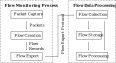
\includegraphics{figures/flow-monitoring-process}
  \end{center}
  \caption{High Level Flow Monitoring Schema}
  \label{fig:flow-monitoring-process}
\end{figure}

This rest of section explains basic terminology and components of the flow monitoring architecture and describes the most commonly deployed flow monitoring architectures.

\subsection{Terminology}

The IPFIX working group published several documents where the architecture for IP Flow Information Export is described~\cite{rfc5470, rfc6183}. However, the terminology used in these documents is not commonly used by the flow monitoring community and some of the terms have different meaning depending on a context. We start by presenting the IPFIX reference model as described in RFC5470~\cite{rfc5470}, which can also be used to describe generic flow monitoring architecture. Then we identify the terms that are often used with different meaning and explain how these terms are used throughout this thesis.

We provide the IPFIX terminology definitions from RFC 7011~\cite{rfc7011} here for the convenience of the reader:

\begin{displaycquote}{rfc7011}[Specification of the IP Flow Information Export (IPFIX) Protocol for the Exchange of Flow Information]

	\begin{description}[style=nextline]
		\item[Observation Point]
      An Observation Point is a location in the network where packets
      can be observed.  Examples include a line to which a probe is
      attached; a shared medium, such as an Ethernet-based LAN; a single
      port of a router; or a set of interfaces (physical or logical) of
      a router.

      Note that every Observation Point is associated with an
      Observation Domain (defined below) and that one Observation Point
      may be a superset of several other Observation Points.  For
      example, one Observation Point can be an entire line card.  That
      would be the superset of the individual Observation Points at the
      line card's interfaces.
      
		\item[Observation Domain]
      An Observation Domain is the largest set of Observation Points for
      which Flow information can be aggregated by a Metering Process.
      For example, a router line card may be an Observation Domain if it
      is composed of several interfaces, each of which is an Observation
      Point.  In the IPFIX Message it generates, the Observation Domain
      includes its Observation Domain ID, which is unique per Exporting
      Process.  That way, the Collecting Process can identify the
      specific Observation Domain from the Exporter that sends the IPFIX
      Messages.  Every Observation Point is associated with an
      Observation Domain.  It is RECOMMENDED that Observation Domain IDs
      also be unique per IPFIX Device.

		\item[Packet Treatment]
      "Packet Treatment" refers to action(s) performed on a packet by a
      forwarding device or other middlebox, including forwarding,
      dropping, delaying for traffic-shaping purposes, etc.

		\item[Metering Process] 

      The Metering Process generates Flow Records.  Inputs to the
      process are packet headers, characteristics, and Packet Treatment
      observed at one or more Observation Points.

      The Metering Process consists of a set of functions that includes
      packet header capturing, timestamping, sampling, classifying, and
      maintaining Flow Records.

      The maintenance of Flow Records may include creating new records,
      updating existing ones, computing Flow statistics, deriving
      further Flow properties, detecting Flow expiration, passing Flow
      Records to the Exporting Process, and deleting Flow Records.
      
		\item[Exporting Process]
      The Exporting Process sends IPFIX Messages to one or more
      Collecting Processes.  The Flow Records in the Messages are
      generated by one or more Metering Processes.

		\item[Exporter]
      A device that hosts one or more Exporting Processes is termed an
      Exporter.

		\item[IPFIX Device]
      An IPFIX Device hosts at least one Exporting Process.  It may host
      further Exporting Processes as well as arbitrary numbers of
      Observation Points and Metering Processes.

		\item[Collecting Process]
      A Collecting Process receives IPFIX Messages from one or more
      Exporting Processes.  The Collecting Process might process or
      store Flow Records received within these Messages, but such
      actions are out of scope for this document.

		\item[Collector]
      A device that hosts one or more Collecting Processes is termed a
      Collector.
    \end{description}

\end{displaycquote}


The Figure~\ref{fig:ipfix_reference_model} shows various scenarios of flow monitoring architecture as defined by IPFIX working group. IPFIX exporters and IPFIX devices are part of the flow monitoring process, collectors and application represent flow data processing, as described in the Figure~\ref{fig:flow-monitoring-process}. The IPFIX Reference Model allows to differentiate between devices that only export flow records and devices that receive data from an observation point and perform the metering process themselves. This can be useful for describing for example development setups where flow records are replayed or generated without the necessity for monitoring of live network traffic. Collectors comprise of collecting processes and data processing applications. The reference model shows that it is possible to collect flow records from multiple sources on a single collector and that the applications can run on directly on the collector or that they can be distributed to other machines. For example, collecting process might convert the flow records in IPFIX format to JSON and feed a big data processing framework that runs on a cluster of machines.

\begin{figure}[t!]
  \begin{center}
    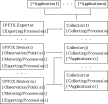
\includegraphics[width=0.7\textwidth]{figures/ipfix-reference-model}
  \end{center}
  \caption{IPFIX Reference Model~\cite{rfc5470}}
  \label{fig:ipfix_reference_model}
\end{figure}

Although the IPFIX Reference Model describes the flow monitoring architecture in detail, it is not used by the flow monitoring community unanimously. Most of the terms used in the IPFIX standard are simplified and their true meaning often depends on the context. Table~\ref{tab:flow_monitoring_terminology} provides the common terms often used instead of the IPFIX terminology. Examples of use of the \Index{common terminology} can be found for example in~\cite{Hofstede-2014-Flow, Cejka-2015-Using, Brownlee-2011-Flow, Krmicek-2009-Netflow, Lee-2007-End, Lee-2007-IPv6, Molina-2006-Design}. We usually talk about a monitored link and a set of monitored links (e.g. both directions of a network connection when optical fibres are used) instead of an observation point or an observation domain. By an exporter or a flow exporter is usually meant the software that performs flow monitoring (both metering and exporting process). If a device generates flows without observing and processing the packets first (i.e. Exporter in IPFIX terminology) we call it a flow source or a probe. The IPFIX Device is usually called by more specific name, such as switch, router, or, in case of a dedicated device possibly with specialized hardware and software equipment, a probe. However, term flow source can also be used for any device that generates flow records. Finally, both the software for collecting flow records and device where such a software runs is commonly called a collector, or a flow collector. We will be using the common terminology throughout this thesis.

\begin{table}[t!]
	\centering
	\begin{tabular}{ll}
	\toprule
		\textbf{IPFIX Terminology}  & \textbf{Common Terminology}                 \\ \midrule
		Observation Point   &  Monitored Link, Observed Link                      \\
		Observation Domain  &  Set of Monitored Links                             \\
		Packet Treatment    &  Packet Treatment                                   \\
		Metering Process    &  (Flow) Exporter [software]                         \\
		Exporting Process   &  (Flow) Exporter [software]                         \\
		Exporter            &  Flow Source, (Flow) Probe                          \\
		IPFIX Device        &  Flow Source, (Flow) Probe, Switch, Router, \ldots  \\
		Collecting Process  &  (Flow) Collector [software]                        \\
		Collector           &  (Flow) Collector [device]                          \\ \bottomrule
	\end{tabular}
	\caption{Flow Monitoring Architecture Terminology}
	\label{tab:flow_monitoring_terminology}
\end{table}


\subsection{Flow Monitoring Deployment}

The deployment of flow monitoring requires careful planning so that it does not disturb the existing network infrastructure. There are several decision that must be made such as choosing a proper flow source, collector and their location relative to the monitored network. Although it is possible to monitor wireless and virtual networks, we focus on the deployment in wired networks.

The selection of the flow source depends upon many variables, such as cost, required quality of exported data, or the type of the monitored link. Two types of flow source are generally available. First are the active networking devices that are already present in the network and provide flow monitoring functionality as well. Switches, routers and firewalls belong to this category. When such a device is present at a convenient point in the network, it must only be properly configured for flow export and no adjustments to the network are needed. Moreover, internal information such as IP addresses behind NAT (Network Address Translation), which would be difficult to access otherwise, can be added to exported flow records. The disadvantage of these devices is that flow monitoring is not their primary function and may not be performed correctly under great load (i.e. under an attack). Also the range of supported options and protocols is usually much lower than that of dedicated probes. The reason for deploying a dedicated probe is usually the need for some extra functionality or guarantees that cannot be met by the networking devices. It also allows to separate network configuration and maintenance from network monitoring, which can be useful if they are handled by different divisions of an organization.

The active networking devices observe packets as a part of their function, dedicated probes, however, need to be provided with access to data. There are two ways for probes to observe the data: in \emph{in-line} mode or \emph{mirrored} mode.
\begin{description}
	\item[In-line mode] -- A device in in-line mode is connected directly to the monitored link and has to actively pass the packets in order for the link to function. This is the mode of operation of active network devices such as switches and routers. The advantage is that no other device is necessary to mirror the traffic, however, if the probe fails the operation of the network is disrupted. Moreover, it could introduce significant latency and jitter to the network connection.
	\item[Mirrored mode] -- In the mirrored mode, a copy of network traffic is created and delivered to the probe using dedicated link. The copy can be created either by dedicated TAP (Test Access Point) or an active networking device with the use of a SPAN (Switch Port Analyzer) port. Table~\ref{tab:tap_vs_span} shows differences, advantages, and disadvantages of TAP and SPAN solutions. An analysis of traffic trace artefacts caused by port mirroring was performed by~\citeauthor{Zhang-2007-Traffic} in~\cite{Zhang-2007-Traffic}.
	\begin{description}
		\item[TAP] is a passive splitting mechanism which require in-line installation. However, due to the simplicity of the device (optical TAPs use mirrors and require no power source) and integrated fail-safes (bypass TAPs), the risk of negatively affecting the network is very low. 
		\item[SPAN] is a special port provided by active networking device that provides a copy of traffic passing through the device for analysis and monitoring purposes.
	\end{description}
\end{description}

\begin{table}[t!]
	\centering
	\begin{tabularx}{\textwidth}{XX}
	\toprule
		\multicolumn{1}{c}{\textbf{TAP}}  & \multicolumn{1}{c}{\textbf{SPAN}} \\ \midrule[1pt]
		
		\multicolumn{2}{c}{Differences} \\ \midrule
		\begin{compactitem}
			\item RX \& TX signal delivered on separate ports
			\item Captures everything on the wire, including MAC and media errors
			\item Complete capture for 100\,\% saturated network
		\end{compactitem}
		&
		\begin{compactitem}
			\item RX \& TX copied into in one TX signal
			\item Hardware and media errors are dropped
			\item Possible packet drop due to SPAN link capacity limit
		\end{compactitem}
		\\ \midrule
		
		\multicolumn{2}{c}{Advantages} \\ \midrule
		\begin{compactitem}
			\item Monitoring device receives identical data, including errors
			\item Keeps link directions separate
		\end{compactitem}
		& 
		\begin{compactitem}
			\item Low cost 
			\item No changes to network topology
			\item Aggregation of multiple links
		\end{compactitem}
		\\ \midrule
		
		\multicolumn{2}{c}{Disadvantages} \\ \midrule
		\begin{compactitem}
			\item Analysis device may need dual-port capture interface
			\item Additional costs for TAP
			\item Necessity to install additional device
		\end{compactitem}
		& 
		\begin{compactitem}
			\item Packet drop on fully utilized full-duplex links
			\item SPAN port data has lower priority than port-to-port data
			\item Some analyses require observation of physical layer errors
			\item Loss of information about link
			\item Increased switch CPU utilization
			\item Can change a timing of frames
		\end{compactitem}
		\\ \bottomrule
	\end{tabularx}
	\caption{Differences Between TAP and SPAN Mirroring Options}
	\label{tab:tap_vs_span}
\end{table}

Since flow monitoring is a passive form of monitoring in its nature, it is a good practice to mirror the live traffic and provide only a copy of the data to the probe so that the network cannot be affected by the monitoring process. Selection of the mirroring technology needs to be considered for each deployment based on specific requirements and limitations, such as utilization of the measured network and impact of packet drop on the performed analysis. The Figure~\ref{fig:flow_monitoring_deployment} shows the most common deployment of flow monitoring at the edge of the network using both presented options: flow export directly from the router and dedicated probe with data provided either by TAP or by router SPAN port.

\begin{figure}[t!]
  \begin{center}
    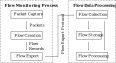
\includegraphics[]{figures/flow-monitoring-deployment}
  \end{center}
  \caption{Flow Monitoring Deployment Schema}
  \label{fig:flow_monitoring_deployment}
\end{figure}

Location of the flow source in the network is very important. When the monitored network is connected to the outside at multiple points, it is necessary not only to monitor each of the points, but also to be sure that the routing policies are reasonable so that packets of each flow traverse only one of these points. The flow source would have to have access to all links and monitor them as a single source otherwise, which is not easily achieved especially when the connection points are geologically distributed. It is a good practice to keep the information about which flow source exported which flow records on the collector so that possible configuration problems are easier to detect.

When monitoring a large network such as a network of an university campus, multiple flow sources can be utilized to gain more detailed information about traffic of individual faculties. Special care needs to be taken when a packet traverses multiple observation points. Counting the same traffic multiple times can have a negative impact on subsequent data analysis.

Deployment of NAT impedes network visibility. Some routers that perform the address translation are able to export both original and translated addresses in the flow records. However, observation points of dedicated flow probes are located either before or after the network device which performs the translation. Although some effort has been dedicated to detection of NAT from data provided in flow records~\cite{Abt-2013-Passive, Krmicek-2009-Netflow}, if does not solve the problem of finding the correct source of the communication behind the NAT. The correct approach would be to either place a second probe to a location where the internal addresses are still visible or to export the information about translation to the collector and pair it with existing flow records.


\section{Flow Monitoring Process}\label{sec:flow-monitoring-process}

This section aims to describe the process of converting raw packets and corresponding packet treatment information to flow records. We show how the flow selection function from Definition~\ref{def:flow-selection-function} relates to this process. For the purposes of this thesis, we will consider dedicated probes equipped with a flow exporter software from now on. Although the the flow monitoring process in networking devices is similar, it has differences and specifics that are outside the scope of this work. This section provides generic overview of the flow monitoring process, performance related details are left for Chapter~\ref{chap:flow-monitoring-performance}.

The Figure~\ref{fig:flow_monitoring_process_detail} shows a common flow monitoring process and its individual parts, which are discussed in the rest of this section. Alternative description of the flow monitoring process can be found in the IPFIX Reference Model~\cite{rfc5470}. We will refer to this description where appropriate.

\begin{sidewaysfigure}
  \begin{center}
    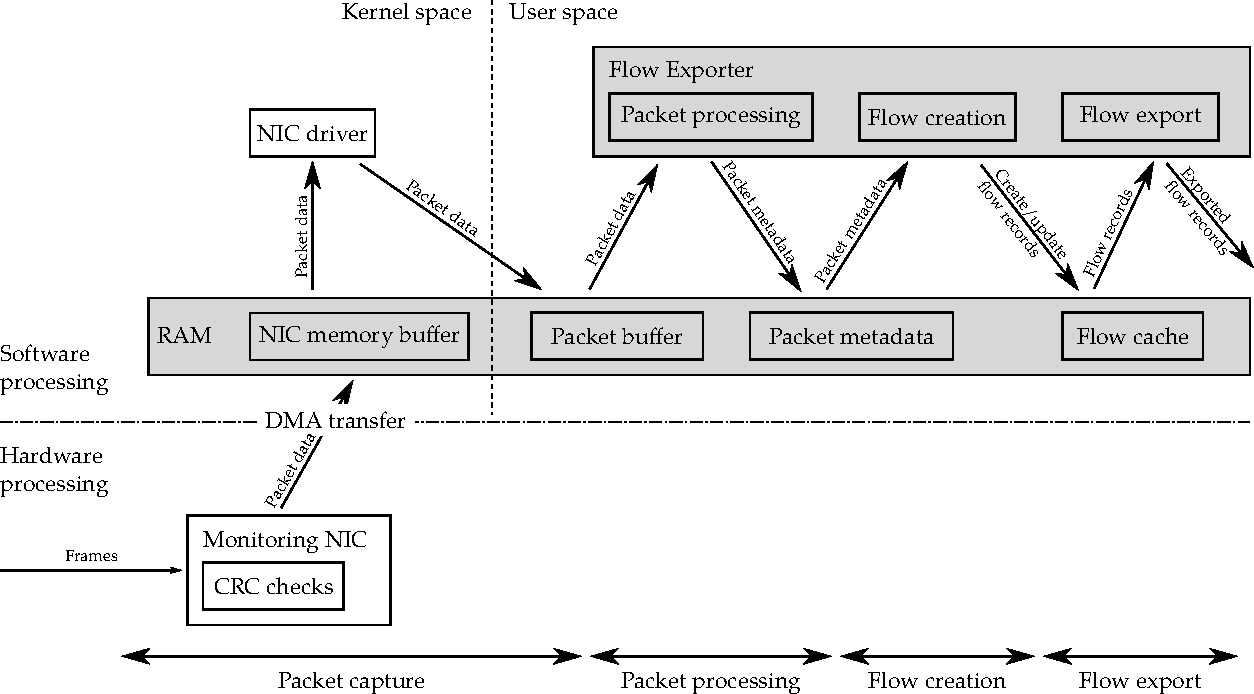
\includegraphics[width=\textheight]{figures/flow-monitoring-process-detail}
  \end{center}
  \caption{Detailed Overview of the Flow Monitoring Process in a Dedicated Probe}
  \label{fig:flow_monitoring_process_detail}
\end{sidewaysfigure}

\subsection{Packet Capture}

The \Index{packet capture} ensures that data from the network are made available for processing in the software. Standard Network Interface Cards (NICs) can be used, as well as specialized hardware accelerated cards. The schema shows a standard NIC performing a CRC check on received packets. The NIC has to be put in a special monitoring mode in order to receive packets with different destination MAC addresses. These packets are passed to the NIC driver, usually through Direct Memory Access (DMA). The driver either passes the received packets to the operating system or provides it's own application interface for accessing the packets from user space. The performance of the different approaches differ significantly and we will discuss it in Chapter~\ref{chap:flow-monitoring-performance} in detail.

Each packet needs to be assigned a (preferably unique) timestamp that marks the point in time at which the packet was received. This process is called packet timestamping. The timestamp can be assigned by the NIC, NIC's driver (or OS), or the software application processing the packet. The support for NIC timestamping is provided by some of the hardware accelerated NICs. As the timestamping in software can be potentially computationally intensive, we will also discuss it in Chapter~\ref{chap:flow-monitoring-performance}.

The packet treatment information is provided together with the packets by the NIC's driver. Usually the interface of NIC on which the packet was captured and the timestamp of the capture is available at least. Networking devices can provide more information such as egress interface, next hop, or autonomous system number of the destination. This information is not directly available when dedicated probes are used, but can be added externally if necessary.

\subsection{Packet Processing}\label{subsec:packet-processing}

The task of the \Index{packet processing} is to extract values of chosen properties of individual packets and corresponding packet treatment information. Attributes such as IP addresses, transport protocol, and ports are used as \emph{flow keys}. The set of used flow keys depend on the applied flow selection function which is used to decide to which flow the packet belongs to. Other attributes of the packets such as TCP flags or number of bytes, are extracted as well for further analysis. We call the extracted properties \emph{\Index{packet metadata}} or \emph{\Index{partial flow records}}. The packet metadata are passed to flow creation part of the flow processing where it is used to create new or update existing flow records.

Secondary task of packet processing is packet sampling and packet filtering, as mentioned in~\cite{rfc5470}. Packet sampling is usually done to reduce the amount of processed data in order to compensate for lack of performance. There are several sampling techniques that can be used as described in~\cite{rfc5476}. Packet sampling is performed before extracting the metadata. Packet filtering can be performed after the metadata is extracted and is based on the extracted values. It is common to monitor only specific network or a section of network, therefore the filtering rules are usually based on extracted IP addresses. Both packet sampling and packet filtering can be implemented in hardware accelerated NICs as well.

\subsection{Flow Creation}\label{subsec:flow-creation}

The extracted packet metadata are aggregated to create flow records. The definition of the flow selection function requires all preceding extended packets of the same flow to determine whether a new packet belongs to particular flow. Since it is not viable to keep all packets of a flow in memory, only selected information is stored in real world implementations. All active flows have a flow record with all necessary information stored in a \emph{\Index{flow cache}}. When a new packet arrives, the flow selection function is called for each stored flow record and the metadata of the new packet to determine, to which flow the new packet belongs. If a matching flow record is found, it is updated using the packet metadata (e.g. packet and byte counters are incremented, flow end timestamp is updated). If no such record exists, the packet is considered to be the first packet of a new flow and a corresponding flow record is created in the flow cache. Algorithm~\ref{alg:flow-record-construction} illustrates the flow creation process. Note that the flow selection function is denoted $\phi$ as we refer to a concrete implementation here instead of the formal definition.

\begin{algorithm}
	\caption{Construction of flow records}
	\label{alg:flow-record-construction}
	\begin{algorithmic}[1]
		\LOOP 
			\STATE Get new packet $P$
			\STATE Extract packet metadata $M$
			\STATE Set \textbf{found} = \FALSE
			\FORALL{flow record $\mathcal{F}$ in flow cache}
				\STATE Apply flow selection function $\phi$ to $\mathcal{F}$ and $M$
				\IF{$\phi(\mathcal{F}, {M}) = true$}
					\STATE Aggregate $M$ to $\mathcal{F}$
					\STATE Set \textbf{found} = \TRUE;
					\STATE \textbf{break}
				\ENDIF
			\ENDFOR
			\IF{\NOT found}
				\STATE Create new flow record $\mathcal{F}$ from $M$
				\STATE Insert $\mathcal{F}$ into flow cache
			\ENDIF
		\ENDLOOP
    \end{algorithmic}
\end{algorithm}

Testing the extracted packet metadata against each flow record has a linear time complexity with respect to to the size of the flow cache. Common optimization is to compute a hash for each flow record such that it can also be computed for the extracted metadata. The flow cache is then either indexed by using the computed hash~\cite{Molina-2006-Design} or directly implemented as a hash table~\cite{Estan-2004-Building} so that the input and lookup operations have a constant time complexity. Collisions can be solved by a number of common techniques or by prematurely exporting the older colliding flow record. This optimization is so widely used that its use is often implicit, but it is important to keep in mind that the new packet is still effectively tested against each active flow. Other implementations of flow caches can be found in literature, such as a hypercube flow table by~\citeauthor{Wang-2011-Memory}~\cite{Wang-2011-Memory}.

There are several reasons why a flow record can exit the flow cache\index{flow!record expiration}{}:
\begin{description}
	\item[Inactive timeout\index{timeout!inactive}] occurs when no new packets belonging to the flow arrive for a time interval called \emph{inactive timeout}. This timeout is used to end inactive connections and has a significant influence on flow cache memory requirements. When set too low the inactive timeout can erroneously split idle connections where keep-alive packet are sent in a longer interval than the inactive timeout. The inactive timeout is sometimes called \emph{idle timeout}\index{timeout!idle} as well.
	\item[Active timeout\index{timeout!active}] occurs when the flow is longer than a time interval called \emph{active timeout}. The reason for active timeout is to keep exported flow information fresh. For example some SSH connections may be active for months when left open in an UNIX/Linux screen utility and without the active timeout the information about the connection would be too late for any practical purpose, such as monitoring the amount of traffic for a given time period. The active timeout is usually much longer than the inactive one. For example, Cisco IOS flow cache has the default of 30 minutes for the active timeout and 15 seconds for the inactive one~\cite{CiscoSystems-2013-Cisco}.
	\item[Natural expiration] occurs when the connection is closed normally. This is often implemented for TCP connections where packets with RST or FIN flag indicate the end of connection.
	\item[Resource constraints] such as lack of memory can cause flow records to be exported from the flow cache to allow new flows to be inserted. Some implementations of flow caches using hash tables have fixed number of flows that can be stored under single hash. Therefore, when a new flow record needs to be created one of the existing flow records is usually expired.
	\item[Exporter shutdown] usually causes all flow records in the flow cache to be exported so that the information about observed packets is not lost. This cause is not often mentioned in the literature, however, we consider it an important one. The exporter must be restarted each time a configuration is changed unless it supports dynamic reconfiguration, which none of the open-source exporters does. Therefore the exported shutdown can happen surprisingly often.
\end{description}

The RFC 5470~\cite{rfc5470} considers both timeouts and resource constraints as causes for a flow record to expire but omits natural close of connection and the possibility of exporter shutdown. Flow record expiration setting can significantly influence not only the  number of generated flow records, as shown by the authors of~\cite{Rodriguez-2013-Empirical}, but also further flow processing and various flow-based detection methods. Implementation of flow record expiration has an impact on the overall flow monitoring performance. Periodically checking the flow cache for expired flows can create latency in packet capture that may result in packet loss. Several approaches to this problem are described in the work of \citeauthor{Molina-2006-Design}~\cite{Molina-2006-Design}.

Little attention has been given to the measurement of traffic with fragmented packets. Although the ratio of fragmented packets is decreasing~\cite{Murray-2012-State}, it is still very important to monitor them since it is quite easy for an attacker to hide an attack from intrusion detection systems by fragmenting the attack packets~\cite{Cheng-2012-Evasion}. The RFC 3917 which describes requirement for IP flow information export states the following about packet fragmentation:

\begin{displaycquote}{rfc3917}[Requirements for IP Flow Information Export (IPFIX)]
   In case of IP packet fragmentation and depending on the
   classification scheme, only the zero-offset fragment of a single
   initial packet might contain sufficient information to classify the
   packet.  Note that this fragment should be the first one generated by
   the router imposing the fragmentation [RFC791], but might not be the
   first one observed by the IPFIX device, due to reordering reasons.
   The metering process may keep state of IP packet fragmentation in
   order to map fragments that do not contain sufficient header
   information correctly to flows.
\end{displaycquote}

This means that the flow monitoring system implementing the IPFIX standard is not required to handle fragmented packets. Moreover, neither the Netflow v9 nor the IPFIX flow definitions cover the possibility to assign a packet fragment to the correct flow, because they require that the common properties are derived from the single packet and the corresponding packet treatment. This is the main reason that the Definitions~\ref{def:flow} and~\ref{def:formal-flow} allow to derive the common properties from data contained in previous packets of the same flow as well. We assume that the packets arrive in the appropriate order for the purpose of these definitions.

Let us consider what happens when an IPv4 packet is fragmented (the problem is very similar for IPv6). Figure~\ref{fig:fragmented-flow} illustrates this scenario. When the packet $K$ is fragmented, its payload is distributed between several different packets $(K\#1, K\#2, \ldots, K\#M_K)$. Only the first packet $(K\#1)$ contains the transport header, others only carry a flag identifying the fragment and offset of the data in the original packet. When a flow record is created for the first part of the fragmented packet, it contains IP addresses, transport layer information (protocol and ports), and the first part of application payload. However, subsequent parts contain only information about IP addresses and consecutive parts of the application payload. The transport level information was already sent in the first fragment. Therefore, flow records created from the subsequent fragments are not aggregated with the first fragment. Moreover, flow records created from subsequent fragments from different connections between the same hosts are aggregated together. To resolve this problem, some kind of packet reassembly must happen either in the flow cache or during packet capture (e.g. packet reassembly at the OS network stack).

A possible solution that has been successfully deployed in practice is to create temporary flow records for fragmented packets where fragmentation identifiers are part of the flow key instead of transport layer information. Therefore, each fragmented packet has its own temporary flow record. By assigning shorter inactive timeout to these flow records the temporary flow record can be reinserted into the flow cache when all fragments are received. This allows to effectively reassemble the original packet with proper transport layer information, which is available since it was present in the first fragment, in the flow cache. The advantage of this solution is that it allows to count number of reassembled packets as well as the number of packet fragments, which can be used in later analyses.

\begin{figure}[ht!]
  \begin{center}
    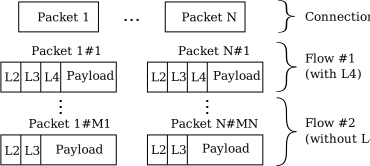
\includegraphics{figures/fragmented-flow}
  \end{center}
  \caption{Flow measurement of a fragmented connection.}
  \label{fig:fragmented-flow}
\end{figure}

The flow monitoring implementation based on flow caches of networking devices kept a separate flow for each direction of a network connection. The reason was that each direction usually had different at least  ingress and egress interfaces. However, for network monitoring and analysis purposes, it is often useful to be able to access flow records for both communication directions at the same time. For this reason the bidirectional flow export was proposed in 2005 and resulted in publication of RFC 5103~\cite{rfc5103} in 2008. The document proposes to aggregate flow records for both forward and reverse directions to a single flow record. Bidirectional flow is called \emph{\Index{biflow}} and unidirectional flow is called \emph{\Index{uniflow}}. The flow keys that are associated with a direction (e.g. source IP address) are called \emph{directional flow keys}. When the biflow record is created, some information must be stored for both directions (e.g. number of bytes and packets) and some information is common to both directions (e.g. flow keys). When biflows are used, the corresponding flow records stored in the flow cache become biflow records as well. Note that creation of biflows is permitted by the definitions NetFlow v9 and IPFIX as well as the Definition~\ref{def:flow}. Although we work mostly with the uniflow in the context of this thesis, most of the concepts apply to the biflow as well. We will mention explicitly when there are important differences between uniflow and biflow.

\subsection{Flow Export}

The flow export manages the process of delivering flow records to flow collectors. The process consists of several parts as shown in the Figure~\ref{fig:flow-export}. The flow sampling and filtering process is very similar to packet sampling and filtering described in the Subsection~\ref{subsec:packet-processing}. The main motivation for flow filtering is that each collector might want to process only a subset of data, e.g. from a particular subnet. The flow sampling is performed when the performance of the collector is not sufficient to process all flow records. The main difference between packet sampling and flow sampling is that the flow sampling always discards whole flow record while the packet sampling can discard some packets of the flow, therefore affecting the created flow record. 

\begin{figure}[ht!]
  \begin{center}
    \includegraphics[width=\textwidth]{figures/flow-export}
  \end{center}
  \caption{Flow export schema.}
  \label{fig:flow-export}
\end{figure}

The flow export protocols such as NetFlow or IPFIX describe how to serialize a flow record and how to use different transport protocols such as UDP, TCP and SCTP to transfer the encoded data to the collector. The NetFlow~v5 and v9 protocols are still widely used although the IPFIX protocol is achieving wide deployment since it offers more features and supports proprietary information elements as well as variable length information elements. Different flow export protocols developed by other vendors can be used as well, as described in Subsection~\ref{subsec:history-of-flow-monitoring}.

The UDP transport protocol is used very often to carry flow records since it was the only one supported by NetFlow. IPFIX specifies the use of TCP and SCTP protocols for flow export as well as the use of the UDP protocol. Although SCTP is mandatory for IPFIX implementations, its real-world usage is hindered by lack of support in software and hardware. When a reliable transport is necessary, TCP is the most often used protocol. For more information about IPFIX transport protocols see RFC 7011~\cite{rfc7011}. A comprehensive comparison of IPFIX transport protocols is also provided in~\cite{Hofstede-2014-Flow}.

Flow records can be exported in many formats over different transport protocols. With the increasing popularity of big data tools such as Kafka, Elasticsearch, Apache Spark, and Hadoop, the need for an universal and widely supported format is more crucial then ever before. As most of the big data tools support JSON, flow records are often transported and stored in the JSON format. The main advantage of JSON is that the data are stored in key-value format without the need to specify templates for the data beforehand. The obvious disadvantage is the increase in the message size due to the need to provide a key for every value in every flow record. It is not unusual for the JSON encoded messages to be more than 7 times larger than in the IPFIX format.

An important part of flow export is ensuring security of the exported flow records. The records must reach only the authorized destination without being observed by any third party. Therefore, authorization, confidentiality and, preferably, also integrity should be provided. The same applies to flow collectors during the collecting process. More information about flow transmission security is provided in Subsection~\ref{subsec:flow-collection}.

\section{Flow Data Processing}\label{sec:flow-data-processing}

The aim of this section is to outline the processing of flow data after they are exported to a flow collector. Firstly, we describe the flow collection process in Subsection~\ref{subsec:flow-collection}. The reception of flow data is not a difficult task itself, but requires several important choices to be made, such as what flow export protocols will be supported and how to handle unknown information elements. Secondly, the flow data are often stored for future needs. The choice of a flow data storage format is very important since the data is written once, read many times and fast searches are required. This process is described in Subsection~\ref{subsec:flow-storage}. Lastly, the flow records are processed and analysed, either by reading the previously stored data or in real time as they arrive from a flow exporter. The flow record processing and analysis is discussed in Subsection~\ref{subsec:flow-processing}. The whole flow data processing schema is shown in Figure~\ref{fig:flow-processing-details}.

\begin{sidewaysfigure}
  \begin{center}
    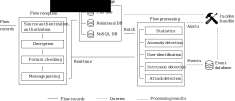
\includegraphics[width=\textheight]{figures/flow-processing-details}
  \end{center}
  \caption{Flow data processing schema.}
  \label{fig:flow-processing-details}
\end{sidewaysfigure}

\subsection{Flow Collection}\label{subsec:flow-collection}

Flow collection is a process of receiving flow records from an exporter performed by a flow collector. The collector and the exporter must choose an appropriate combination of transport protocol and flow export protocol before the data transmission starts, there is no protocol for flow export parameters negotiation. Although the collector can receive data using a multiple combinations of protocols at the same time, such feature is not usually implemented due to added complexity.

After the collector validates that a received message is in the expected format, it attempts to parse individual flow records. This process may vary for each flow export protocol, however, the collector always needs to derive correct data types of information elements in order to be able to work with them. The common practice with NetFlow information elements was to hardcode their definitions and extend the code every time it was necessary to add a new element. The extensibility of the IPFIX protocol information elements through the use of Private Enterprise Numbers advocates more dynamic approach to information element handling, although a subset of IPFIX information elements are sometimes hardcoded as well. Since the collectors cannot know all possible information elements that can be sent by exporters, it is necessary to correctly handle new and unknown elements. Although they are usually discarded, it is also possible to process them when their data types can be derived from the information provided by the flow export protocol.

When using NetFlow and IPFIX protocols in combination with the UDP transport protocol it is necessary to properly manage templates messages containing the definitions of flow record formats. The templates can change during the collection process, e.g. after exporter restart, and it can easily result in incorrectly decoded messages. The IPFIX protocol specification~\cite{rfc7011} describes how the template messages should be handled and what to do in case of missing templates. Both NetFlow and IPFIX protocols keep track of lost messages by assigning a sequence number to each message. NetFlow~v5 increase the sequence number for each transmitted flow record, which allows to keep track of the number of lost flow records. This behaviour was changed in NetFlow~v9 so that the sequence number is increased for each transmitted NetFlow~v9 packet. It is more difficult to keep track of the number of lost flow records in NetFlow v9, but easy to see how many packets were lost, which can help with determining the cause of the packet loss. The IPFIX protocol increments the sequence number per flow record, just like NetFlow~v5. However, when a template is missing, it is not possible to determine the exact number of flow records in a packet, therefore the collector cannot be sure whether flow records were lost during the transmission or not. This is one of several reasons to use IPFIX over a reliable channel.

An important and often neglected aspect of flow collection is security. The collector needs to authenticate the source of the data to avoid processing of malicious flow records or malformed messages intended to attack the collector itself. There are several ways to authenticate the source of the data. IP addresses can be used to authenticate the flow exporter and the collector itself or a firewall can be set to allow data from authorized IP addresses. However, this does not prevent attackers with the ability to spoof IP addresses when UDP transport protocol is used. Moreover, the Man-in-the-middle (MITM) attack cannot be prevented without an appropriate use of cryptography. Proper authentication, usually using certificates, is needed to mitigate the MITM attack. The IPFIX protocol requires that TLS version 1.1 is implemented for TCP and DTLS 1.0 for STCP and UDP procols. Moreover, it requires mutual authentication when using TLS or DTLS so that the exporter does not send sensitive data to an unknown target. Table~\ref{tab:flow.protocols.security} shows how IP spoofing and MITM attack are mitigated by use of TLS and DTLS protocols. The advantage of TLS and DTLS protocols is that they provide not only authentication, but also integrity and confidentiality. Since an IP address is often considered to be a sensitive information, ensuring confidentiality of flow records during transmission should be considered a necessity.

\begin{table}[t!]
	\centering
	\begin{tabular}{lll}
	\toprule
			& \textbf{IP Spoofing}	& \textbf{Man-in-the-Middle}  \\ \midrule
	UDP		& yes			& yes \\ 
	TCP		& no			& yes \\ 
	SCTP		& no			& yes \\
	DTLS/UDP	& no			& no  \\
	TLS/TCP		& no			& no  \\ 
	DTLS/SCTP	& no			& no  \\ \bottomrule
	\end{tabular}
	\caption{Applicability of IP spoofing and MITM attack to transport protocols}
	\label{tab:flow.protocols.security}
\end{table}

Although the IPFIX protocol requires implementation of TLS and DTLS protocols, not every flow exporter and collector supports it. There are two often used solutions for ensuring security of flow record transmission. The first is to build secure channel between exporters and collectors using external tools, such as virtual private networks or stunnel~\cite{Trojnar-2015-Stunnel}. The second solution used in networks that are fully under control of the administrator is to place the exporter and collector in a dedicated network (using private IP addresses) so that they can be accessed only from allowed and trusted address range.


\subsection{Flow Storage}\label{subsec:flow-storage}

There are many uses for flow data~\cite{Li-2013-Review, Umer-2017-Flow}. At first the data were being used for traffic accounting and flow records are often kept by telecommunications companies to comply with laws requiring them to store communication records nowadays. Companies and even individuals also keep flow records of their own traffic so that they can investigate breaches and other security issues ex-post. To store the flow data records for a long period of time, the selected data storage format must be space efficient. Another important aspect of flow data storage is its query performance. The requirements for the query performance differ depending on a particular use case. When overall statistics are requires, all flow records need to be accessed. In case of a security breach investigation, filters for particular IP addresses and ports are likely to be used so that it is beneficial for the data storage to have some kind of index built on the data.

There are several types of data storage that are used for flow data. Firstly, the data can be stored in a flat file without indexes. This approach is utilized by popular flow data manipulation frameworks SiLK~\cite{Shimeall-2014-Using} and NFDUMP~\cite{Haag-2014-NFDUMP}. The main advantage is that the format is very simple and the data is efficiently encoded. Moreover, both file formats support compression which allows for more disk space to be saved. Flat files also take advantage of the fact that flow data is never updated so the records can be tightly packed.

A second popular approach is to store flow data in a relational database. In case of NetFlow~v5, a single table serves to store all flow records. However, when multiple templates are used for the flow records, such as in NetFlow~v9 and IPFIX protocols, the number of tables grows and the relational model becomes complicated. Since relational databases are designed to support much more features than needed for flow data (e.g. updates or complex joins) and often lack support for network data types such as IP and MAC addresses, their performance and disk space requirements are often worse than that of flat files, as shown by \citeauthor{Hofstede-2010-Network} in~\cite{Hofstede-2010-Network}.

The last approach is to use a NoSQL database to store flow data. Although NoSQL databases do not offer as many features as relational databases, they are meant to be able to handle huge amounts of data. A category of NoSQL databases are columnar databases. Instead of storing each flow record as a single database record, it stores each element of the record in a separate file. The benefit of this approach is that, for example, when a query for a certain IP address is evaluated, only files with IP addresses need to be searched. Other requested elements are read from their own files as necessary after the address is found. This approach reduces the amount of data that needs to be read from the disk, however, it causes more random accesses than when using flat files. More information about comparing flat file approach with a NoSQL columnar database is provided in Chapter~\ref{chap:next-generation-flow}. Document oriented databases are also a class of NoSQL databases and their popularity has been increasing lately. Although the performance of most document oriented databases is not sufficient to handle flow data from large networks, they are used for their flexibility that allows for building prototype analytics applications very quickly. The advantage of document oriented databases is that the different structure of flow records is of no concern to the database as it considers each entry to be a generic document. Elasticsearch~\cite{Gormley-2015-Elasticsearch} is a good example of a such a database.

The list of used approaches is by no means complete. There are many Big Data analytics frameworks, that are being used for flow data storage and analytics, such as Hadoop~\cite{Lee-2012-Toward}. Although it is possible to use almost any data storage for flow data, it is difficult to select the best one, since the criteria differ for each use case. It is for that reason, that companies use different flow data storage or develop their own solution in their products.


\subsection{Flow Processing}\label{subsec:flow-processing}

Large amount of information about network traffic and communicating parties can be acquired by a flow record analysis. Many intrusion detection systems use flow records as their primary source of data, especially since deep packet inspection is being made difficult due to the increasing ratio of encrypted traffic. The flow data analysis can be performed either using the stored data or in real time.

When the flow record analysis is performed on stored data, the processing is usually done in batches. The flow collector usually partitions the data according the time of arrival so that once a partition is finished, it can be processed in a single batch. Five minute long time windows are often used as this is the default time interval employed by the popular flow processing tool NfSen~\cite{Haag-2011-NfSen}. The advantage of this approach is that the processing can easily be repeated on the same data, which allows the user to fine-tune the queries and analyse the data on demand. The processing can also be postponed when the system is under heavy load. The disadvantage of batch processing with fixed time intervals is that it introduces delays to data analysis, which can be inconvenient when a rapid action is required based on the results.

When the delay introduced by the batch processing impedes time-critical applications, stream processing can be used instead. In stream processing, the flow records are passed to the processing immediately after they are received. A good overview of the stream-based flow processing is provided by \citeauthor{Jirsik-2017-Toward} in~\cite{Jirsik-2017-Toward}. There is a number of stream processing systems that are used for big data processing. \citeauthor{Cermak-2016-Performance} performed flow data analysis using three most used distributed stream processing systems in~\cite{Cermak-2016-Performance}, and compared their performance. The results show that the distributed stream processing systems are able to scale to accommodate large workloads such as processing of data from very large networks.

The flow processing can be used to achieve several goals. Firstly, both live and long term network statistics can be computed. Live statistics are used by administrators to gain an overview of a network situation. This is useful for tracking down problems and optimizing network configuration when the changes take effect immediately. The long term statistics provide useful information for capacity planning. Secondly, flows can be used to gain situational awareness about the network and connected devices~\cite{Lastovicka-2017-Situational}. This includes device identification and application classification, which often use machine learning techniques for this purpose. Thirdly, flows are nowadays frequently in intrusion detection systems used to detect attackers on network, as described by \citeauthor{Umer-2017-Flow} in~\cite{Umer-2017-Flow}. Lastly, anomaly detection techniques are being applied to flow data to detect suspicious behaviour which might indicate a problem or attack on the network. There are many anomaly detection techniques as surveyed by \citeauthor{Chandola-2009-Anomaly} in~\cite{Chandola-2009-Anomaly} and significant effort was put to applying these techniques to flow data by various researchers.

Modern machine learning techniques are utilized in flow processing. The most common uses are in traffic classification~\cite{Velan-2015-Survey}, user identification~\cite{Verde-2014-No} and intrusion detection~\cite{Tsai-2009-Intrusion}. Although the research in this area is quite extensive, the authors of~\cite{Sommer-2010-Outside} show that the result are seldom applied in practice and provide several observations explaining the difficulties faced by the implementers. A survey of traffic classification techniques for encrypted traffic is provided in Chapter~\ref{chap:measurement-of-encrypted-traffic}.


\section{Common Issues}\label{sec:common-issues}

Although flow monitoring is widely used, there are many not widely known aspects that need to be taken into consideration during its deployment. This section describes several issues that can be encountered in any flow monitoring system and that are easily neglected. We draw mainly from our experience of running the flow monitoring infrastructure of CESNET National Research and Education Network in this section. Most issues concern data loss. Either the data is not correctly observed, parsed, are lost during transmission, or are not interpreted correctly. Firstly, we look at the more obvious and easily detectable issue where no data arrive at all. Then we describe the issues that cause data loss which is not easily detected. Lastly, we discuss issues and misunderstandings that cause the data to be incorrectly measured and interpreted. Let us note here, that a suitable logging facilities of flow exporter and collector together with a reliable log processing mechanism can help to discover many of the described issues.

\subsection{Visible Data Loss}

The usual cause of data loss is that the monitoring infrastructure is misconfigured. Whether it is due to a misconfiguration at the flow exporter or the flow collector side, the obvious indication of the problem is that no data are stored and no results of the flow data processing, such as statistics, are generated. As the problem is quite easily observed, its cause is easily detected. The best way is to review the whole flow processing setup from packet observation to flow storage and processing to see at which point the data are lost.

The first component to investigate is the packet observation. It is possible that the data are no longer sent to the observation point, possibly due to a failed TAP device or a router misconfiguration. This can be easily confirmed using interface packet counters. Even if the data arrive at the observation point, the flow exporter might be configured to read data from from incorrect interface. When the flow exporter is receiving and processing the data, it is important to audit the flow export settings. The data might be sent to incorrect destination or using incompatible transport or flow export protocol. When TLS/DTLS is used, the certificates and keys might not match. It is a good practice to verify that the data actually leave the probe, for example by using a tool such as \emph{tcpdump}.

Since the flow probe is often placed in a dedicated network, it is useful to verify that the network is configured to allow the communication between the probe and the flow collector.

The flow collector must be configured to accept data from the flow exporter, which includes a proper setup of certificates and keys. Even when the flow collector receives the data, it might be running using incorrect configuration and the data might be saved to an unexpected location or not passed to storage and processing at all. A collector may also decide to discard flow records containing unknown information elements. When the flow exporter includes such an element in every record, all flows are dropped. 

\subsection{Unobserved Data Loss}

It is impossible to continuously verify that all observed packets are accounted for in the flow records processed by the flow collector. Since each flow record contains information from packets observed at a different time interval, it is not possible to compute the exact number of packets that passed an observation point from the respective flow data. All statistical information about number of transferred packets are to a certain level biased. The only test that can be continuously applied is that the total number of observed packets at the observation point and at the flow collector remain in a similar range. Since it is not possible to verify that every packet is observed, some packet of even flows might be lost in the flow monitoring process without notice.

There are many networking protocols in use nowadays. Although all flow exporters support the basic protocols such as IPv4, TCP, UDP, and ICMP, they also need to be able to process many data link layer protocols, such as VLAN, VXLAN, MPLS, TRILL, and others. When a new protocol is used on the network for which the flow exporter is not ready, the flow record cannot be created and the information is lost. A similar issue involves tunnelling protocols, such as GRE or protocol 41. For example, when the original IP packet is encapsulated in another L3 protocol, it is important to decide whether the flow record should be created from the inner or outer L3 header. Without an additional mechanism to provide more information about the tunnelled traffic, information from one of the headers is lost.

Flow records containing unknown informational elements might be discarded by the flow collector, as described in the previous section. However, when only some of the flow records contain such information elements, the issue is harder to observe. Therefore it is necessary to have a good knowledge of the used flow collector and its behaviour.

Sometimes messages can be longer than the MTU of the link between the flow exporter and flow collector, especially when application layer information is contained in the flow records. In such a case, use of UDP transport protocol might cause data loss as fragmented packets are sometimes blocked by firewalls. Moreover, the packet loss is more probable since by loosing a single fragment the entire message is unreconstructable and must be discarded. When such a long messages need to be sent, it is best to use a reliable transport protocol such as TCP or SCTP.

One of the most common reasons for data loss in flow monitoring is that the performance of flow exporter or a flow collector is not high enough to process all data. There are several places where either packets or flow records might be dropped, as shown in Figure~\ref{fig:flow-packet-drop}. The first is the source of data for the observation point. When the data to the observation point are provided using router SPAN port, the capacity of the SPAN port must be equal or greater to that of individual links that are measured, otherwise some packet will be dropped by the router when there is a lot of traffic. This is not an issue when using a TAP, because the TAP always splits a single link or a duplex link to two links of the same type and capacity. The second point where packets are often dropped is the observation point. When the exporter does not process the data before the packet reception buffer is full, the newly arrived or the oldest packets are dropped, based on the implementation of the buffer. The third point where the data might be dropped is on the collector device. When the flow collector does not process data quickly enough, the system packet reception buffers fill up and new packets are dropped. This is similar to the packet drop on flow probe, however, every packet lost at the collector contains several flow records that were created from many packets. Therefore, loss of packets with complete flow records is much more serious.

\begin{figure}[t!]
  \begin{center}
    
\includegraphics{figures/flow-packet-drop}
  \end{center}
  \caption{Flow monitoring packet drop schema.}
  \label{fig:flow-packet-drop}
\end{figure}

The choice of transport protocol have an impact on the packet drop as well. UDP messages are discarded by the collector when it does not process in a timely manner. However, using congestion aware protocol such as TCP and SCTP, the collector might create a backpressure on the flow exporter so that it cannot send new messages when it needs to. Therefore,the flow exporter can either drop such messages or wait for the collector to process more data. However, when the flow exporter does not drop the messages, it creates backpressure to flow cache, packet processing, packet parsing and packet reception. This way the slow processing on collector might easily lead to packet drop at the observation point. Another reason for flow exporter not being able to send messages is a slow link between the exporter and collector. When application information is present in the flow records, the required throughput might easily exceed 100\,Mbps, especially when the exporter sends data to multiple collectors. Although such slow links are not used very often nowadays, they might still be encountered in practice.

Although packet drop should be avoided at both flow exporter and flow collector sides, sometimes it is necessary to drop packets in a controlled manner, e.g. under a DDoS attack. We recommend to create a packet buffer in the application to which the data is always stored. Then, when the data processing is slow and the buffer becomes full, the application can decide which packets to drop. The advantage of this approach is that the application is aware of the congestion and can properly react to it, e.g. by reporting it or limiting the processing to a bare minimum.

A very common cause of packet loss at the collector side is the shutdown or restart of flow exporter. The flow exporter usually expires all flow records in the flow cache so that they are not lost. However, as the flow cache may contain hundreds of thousands of flow records, exporting them all at one at the highest possible rate (the flow exporter needs to shutdown or restart without an unnecessary delay) can overwhelm the flow collector. Therefore, it is best to implement two types of shutdown, emergency and graceful. In the emergency shutdown, the data in the flow cache are simply discarded as they are not considered important. This allows to quickly shutdown and restart the exporter, which is beneficial during testing and for important configuration changes. The graceful shutdown should have a configurable flow record export rate. This allows to adapt the capabilities of the flow collector without overwhelming it and limiting the risk of data loss.

Flow monitoring performance is discussed in detail in the Chapter~\ref{chap:flow-monitoring-performance}.


\subsection{Other Issues}

There are other problems that can be encountered during flow monitoring apart from the performance issues and data loss. We have already described the problem with counting lost flow records and elements in The Subsection~\ref{subsec:flow-collection}. This section describes the most common of the issues that cause the data to be incomplete or incorrect.

The first issue is encountered at flow exporters that process biflows. To process biflows correctly, the exporter needs to observe both directions of each flow. There are several reasons why it may fail to do so. Only single direction might be connected to the probe or the network configuration might route the packets asymmetrically. Even if both directions can be observed at the observation point, packets might be received, parsed, and processed in several different queues to speed up the monitoring process. In such a case, it is important to use a correct algorithm to select queues for packets, otherwise the packets from opposite directions may end up in different flow caches and the created biflows will be incomplete. The algorithm must be able to work with all packet headers that precede the headers from which the flow keys are derived. 

Both the flow exporter and flow collector must agree on the semantics of the elements of exported flow records. For example, the packet length is usually exported in IPFIX format as a \emph{octetDeltaCount} element. The specification~\cite{IANA-2017-IP} defines it to be the number of octets since the previous report (if any) in incoming packets for this Flow at the Observation Point. The number of octets includes IP header(s) and IP payload. However, some exporters put the total number of octets including the link layer in this field. Moreover, the IPFIX protocol is sometimes used to export information about non-IP flows as well, so that this element is used differently for specification. Whether the exporter and collector adhere to the specification, it is important the they interpret the semantics equally. In this case, it would be proper to setup a different element with different semantics if the total number of octets needs to be reported.

Different exporters can encode flow record elements to integers, strings and byte arrays of different length. For example, the IPFIX protocol supports \emph{Reduced-Size Encoding}~\cite{rfc7011} which allows encoding elements using fewer octets than the number specified by~\cite{IANA-2017-IP}. Although this saves resources such as memory of the flow exporter, network bandwidth, and disk space on collector, it makes it more difficult to process correctly. When the same element is received by the collector using two different data types, it needs to decide which is going to be used for further processing as maintaining both original data types is cumbersome. The collector usually converts the data to the largest possible data type since it cannot know it advance whether it will receive the element encoded differently in the future and reducing the size of an element may lead to information loss.

The encoding of TCP flags in IPFIX protocol is a good example of issues that can be caused by the \emph{Reduced-size Encoding}. NetFlow~v9 defined TCP flags element as one byte and the IPFIX used single byte as well originally. However, the TCP control bits occupy 9 bites in the TCP header~\cite{rfc3540}, therefore a change was proposed in 2013 to change the encoding to two bytes. The discussion resulted in RFC 7125~\cite{rfc7125} in 2014 with IPFIX supporting the export of TCP flags as a two byte value, as shown in Figure~\ref{fig:tcp-flags}. When reduced size encoding is used only the original byte is exported for backwards compatibility. This presents the authors of flow collectors with a difficult issue. If they support TCP flags as a two byte value, they must indicate that the received element was only a single byte long. Storing two byte value and padding with zeroes is not an option since that would set the ECN nonce sum flag to zero although the collector has no knowledge of its original value.

\begin{figure}
  \begin{center}
    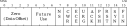
\includegraphics[width=\textwidth]{figures/tcp-flags}
  \end{center}
  \caption{TCP control bits export in IPFIX protocol~\cite{rfc7125}.}
  \label{fig:tcp-flags}
\end{figure}


\section{Conclusions}\label{sec:nfm-conclusions}

This chapter has explained flow monitoring, its history, common uses, and discussed related technologies that are sometimes confused with flow monitoring. We have shown, that the currently used definitions of flow do not reflect the reality of real-world flow monitoring deployment and provided and improved definition that amends the deficiencies. We have also created a formal notation for our definition which allows us to avoid misunderstandings created by the use of informal language. It also allows flow related algorithms to be written more precisely and concisely.

The rest of the chapter has discussed details of the flow monitoring process from the packet capture on a probe to the flow processing on a collector. We have also shown the most common issues that can be encountered while deploying and operating a flow monitoring infrastructure. The most critical issues are caused by incorrect implementation and low performance. We investigate the performance of flow monitoring in Chapter~\ref{chap:flow-monitoring-performance}.
